\tikzstyle{inner} = [thin, circle, minimum size = 0.3cm, draw, inner sep = 0.1pt, black]
\tikzstyle{inner_g} = [thin, circle, minimum size = 0.3cm, draw, inner sep = 0.1pt, black, fill = green]
\tikzstyle{ed} = [thick, ->, draw, black]

    
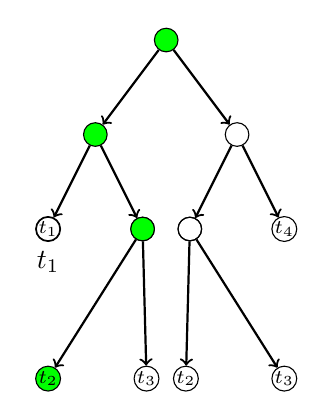
\begin{tikzpicture}
    \node[inner_g] (a) at (0, 0) {};
    \node[inner_g] (b) at (-0.9, -1.2) {};
    \node[inner] (c) at (0.9, -1.2) {};
    \node[inner, label = below:$t_1$] (d) at (-1.5, -2.4) {};
    \node[inner_g] (e) at (-0.3, -2.4) {};
    \node[inner] (e2) at (0.3, -2.4) {};
    \node[inner] (d) at (-1.5, -2.4) {\scriptsize $t_1$};
    \node[inner_g] (e) at (-0.3, -2.4) {};
    \node[inner] (e2) at (0.3, -2.4) {};
    \node[inner] (f) at (1.5, -2.4) {\scriptsize $t_4$};
    \node[inner_g] (g) at (-1.5, -4.3) {\scriptsize $t_2$};
    \node[inner] (h) at (-0.25, -4.3) {\scriptsize $t_3$};
	\node[inner] (g2) at (1.5, -4.3) {\scriptsize $t_3$};
    \node[inner] (h2) at (0.25, -4.3) {\scriptsize $t_2$};
    
    \path (a) edge[ed] (b);
    \path (a) edge[ed] (c);
    \path (b) edge[ed] (d);
    \path (b) edge[ed] (e);
    \path (c) edge[ed] (e2);
    \path (c) edge[ed] (f);
    \path (e) edge[ed] (g);
    \path (e) edge[ed] (h);
    \path (e2) edge[ed] (g2);
    \path (e2) edge[ed] (h2);
\end{tikzpicture}
